This section describes the purpose, use, and intended user audience for the Interactive Degree Planner. The basic concept of this web-based application is to assist UTA Computer Science and Engineering (CSE) students to create their degree planners that best fit their academic path. The website aims to provide the user-friendly interface taking advantage of drag-and-drop to simplify the degree planning process.

\subsection{Purpose and Use}
The Interactive Degree Planner website allows UTA students to register and log into the system. The users need to update their degree information before using the application. They are able to select the latest flow charts from the list of supported majors (i.e., Computer Science, Computer Engineering, and Software Engineering); this allows the website to offer the appropriate course catalog of the right major. Each course option in the provided list includes all important information, such as credit value, course title, course number, course description, and etc. Notably, these options are only available for the users as long as they fulfil the pre-/co-requisite and UTA is going to offer the class in the specific semester. The drag-and-drop pattern is implemented in the hope of facilitating the users' experience during the planning process. The users can freely modify their planners as long as no restriction is violated. Besides, the website  demonstrates essential information, including the total hours per semester and the estimated graduation date.

\subsection{Intended Audience}
The intended audience of this web-based application are current and/or future CSE students at the University of Texas at Arlington. Currently, the website are developed based on only three majors in the CSE department. However, all UTA students, who have different majors, are still able to use this website to build their possible-CSE planner as reference information.

\begin{figure}[h!]
	\centering
   	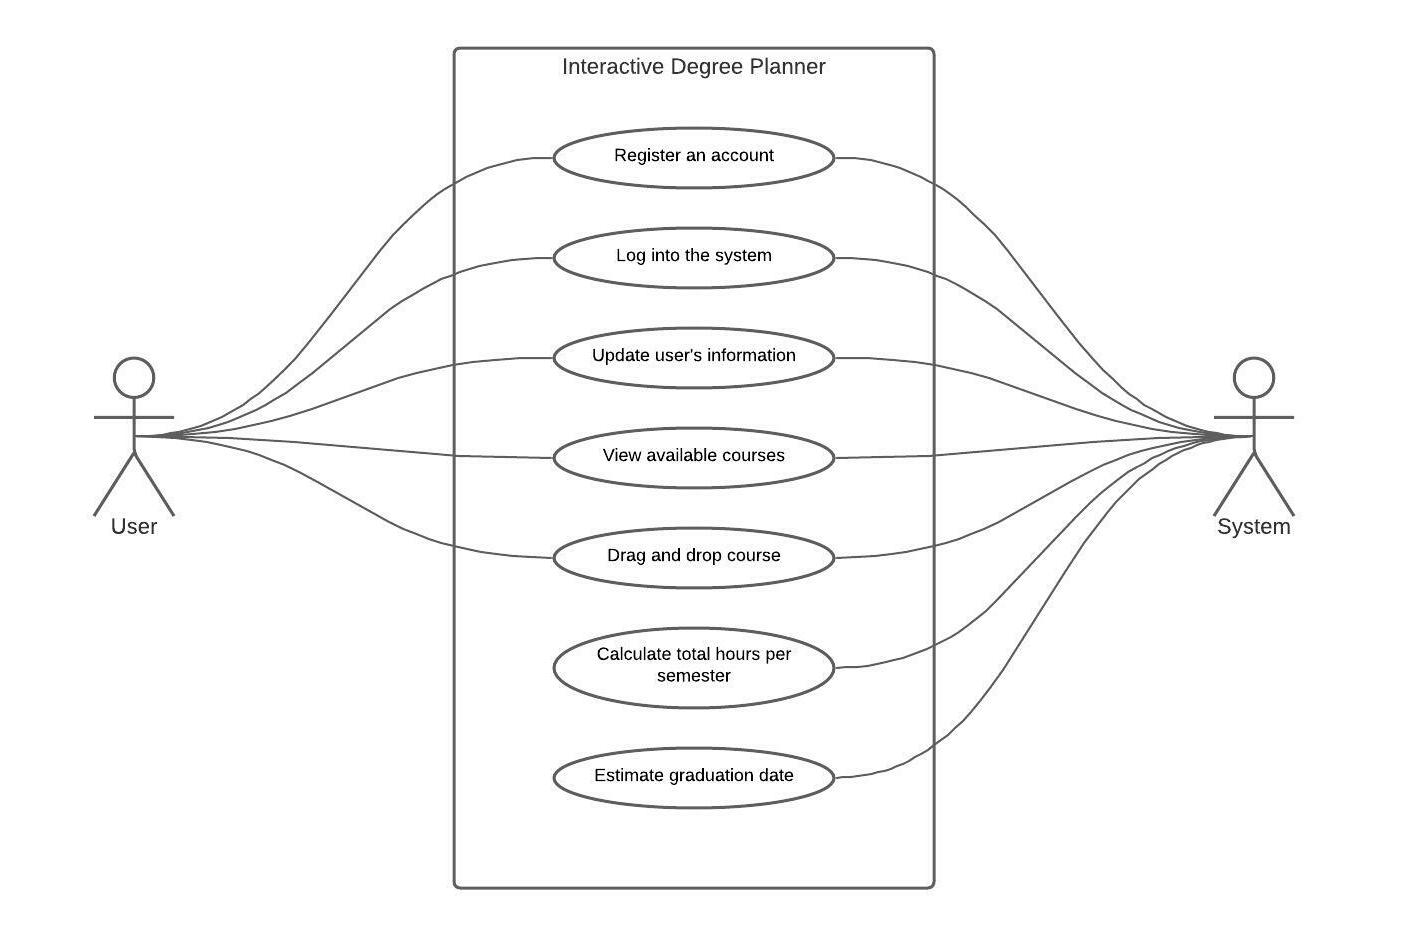
\includegraphics[width=0.60\textwidth]{images/uml}
    \caption{IDP conceptual drawing}
\end{figure}
